%%%%%%%%%%%%%%%%%%%%%%%%%%  phdsymp_sample2e.tex %%%%%%%%%%%%%%%%%%%%%%%%%%%%%%
%% changes for phdsymp.cls marked with !PN
%% except all occ. of phdsymp.sty changed phdsymp.cls
%%%%%%%%%%                                                       %%%%%%%%%%%%%
%%%%%%%%%%    More information: see the header of phdsymp.cls   %%%%%%%%%%%%%
%%%%%%%%%%                                                       %%%%%%%%%%%%%
%%%%%%%%%%%%%%%%%%%%%%%%%%%%%%%%%%%%%%%%%%%%%%%%%%%%%%%%%%%%%%%%%%%%%%%%%%%%%%%


%\documentclass[10pt]{phdsymp} %!PN
%\documentclass[twocolumn]{phdsymp} %!PN
%\documentclass[12pt,draft]{phdsymp} %!PN
%\documentstyle[twocolumn]{phdsymp}
%\documentstyle[12pt,twoside,draft]{phdsymp}
%\documentstyle[9pt,twocolumn,technote,twoside]{phdsymp}
\documentclass[a4paper,oneside,12pt]{article}

\usepackage{pdfpages}
\usepackage{a4wide}
\usepackage[english]{babel} 
\usepackage{url}
\usepackage{caption}
\usepackage{multirow}
\usepackage{rotating}
\usepackage{soul}
 
\usepackage{palatino}

\usepackage{graphicx}
\graphicspath{{figures/}} 
\def\BibTeX{{\rm B\kern-.05em{\sc i\kern-.025em b}\kern-.08em
    T\kern-.1667em\lower.7ex\hbox{E}\kern-.125emX}}

\newtheorem{theorem}{Theorem}

% zet de paragrafen een beetje uit elkaar en links uitgelijnd
\setlength{\parindent}{0mm}
\setlength{\parskip}{1ex plus 0.5ex minus 0.2ex} 

\setlength{\textheight}{23cm}
\setlength{\textwidth}{16cm}
\setlength{\oddsidemargin}{0cm}
\setlength{\evensidemargin}{0cm}
\setlength{\topmargin}{-1cm}

\penalty-10000
\tolerance=10000

% \setlength{\parskip}{0pt}
% \setlength{\parsep}{0pt}
% \setlength{\headsep}{0pt}
% \setlength{\topskip}{0pt}
% \setlength{\topmargin}{0pt}
% \setlength{\topsep}{0pt}
% \setlength{\partopsep}{0pt}

\linespread{0.9725}

\usepackage[compact]{titlesec}
%\titlespacing{\section}{1pt}{*0}{*0}
%\titlespacing{\subsection}{1pt}{*0}{*0}
\titlespacing{\subsubsection}{1pt}{*0}{*0}

\usepackage{mdwlist}

\begin{document}


%-------------------------------------------------------------------------------------------

\thispagestyle{empty}

\begin{center}
\mbox{}\\\vspace{5mm}
{\Large Application for China Scholarship Council Grant}\\ [45mm]
%
{\bf\Huge Hardware acceleration for\\
[3mm] FPGA CAD Tools} \\
\vspace{45mm}
\Large Yun Zhou \\
\vspace{2mm}
\small\texttt{\hl{email@address.com}} \\
\vspace{20mm}
\Large Advisor: ir.\ Elias Vansteenkiste \\
\small\texttt{Elias.Vansteenkiste@ugent.be} \\
\vspace{2mm}
\Large Promotor: prof.\ dr.\ ir.\ Dirk Stroobandt \\
\small\texttt{Dirk.Stroobandt@ugent.be} \\
\vspace{20mm}
\normalsize Ghent University, Belgium \\
\normalsize Department of Electronics and Information Systems\\
\normalsize Computer Systems Lab\\
\normalsize Hardware and Embedded Systems Group 
\end{center}

\newpage

\tableofcontents

\clearpage

\section{Problem Definition \hl{(1 page)}}
A Field Programmable Gate Array (FPGA) is an integrated circuit made up of a grid of programmable functional blocks embedded in a programmable interconnection network. An FPGA can be programmed to implement any arbitrary logic function in the same way as Application Specific Integrated Circuits (ASICs), however the functionality of an FPGA is not fixed during the production process. The functionality can be changed by writing a different configuration to the configuration memory. This flexibility of FPGAs leads to a substantial reduction of the economic risk of developing hardware accelerators. It also explains the rise in the popularity of the FPGA. Unfortunately the flexibility of the FPGA comes at a price.  Each time the application developer wants to test his design, the design has to be compiled to a FPGA configuration and this is a complex and time consuming process. Unfortunately the designer typically needs to compile his application numerous times to test if his/her design meets the constraints of the application. 

The main FPGA device manufacturers and the academic community have developed a chain of heuristics to solve the NP hard problems involved in the compilation.
The compilation/translation of a high-level description of the application to a FPGA configuration is typically divided in several steps. In each step NP hard problems have to be solved and heuristics were and are being developed to try to approximate an optimal solution. The most time-consuming steps are the placement and routing steps. They are the last steps at the backend of the tool flow. These steps have to performed to obtain accurate timing information, which is needed to assess if the design meets the constraints. 
 
Another trend is the increase in both the size of applications and the size of the target devices. FPGA device and application sizes are still increasing following Moore's law~\cite{shannon2015technology}. Unfortunately the power of the FPGA CAD tools lag behind. The traditional CAD heuristics scale very badly in terms of application and device size, which translates to waiting times of hours up until days for compilation to finish \cite{murray2015timing}. 

Since the introduction of high-level synthesis\cite{}, more and more engineers with a software background attempt to accelerate applications with an FPGA. They are used to gcc-like compilation times. Their design methodologies are adapted to these short compilation times. In order to fix bugs and measure performance the compilation is performed numerous times. Hence, they cannot accept the long compilation times that are common in FPGA design.

To overcome this problem, device manufacturers and academics developed multi-threaded versions of the heuristic algorithms \cite{ludwin2011,gort2012,betz2013method,jain2014multi}, but unfortunately scalability issues still exist and large designs still need hours to be compiled. To further speed up compilation a straightforward path is to use hardware acceleration, but unfortunately the current multi-threaded algorithms for placement and routing are hard to adapt for the wide scale parallelisation used in hardware accelerators such as GPUs and FPGAs.

Summary: \emph{FPGA design compilation takes too much time to allow efficient design turnaround times. Hardware acceleration of the compilation process is needed but the current placement and routing algorithms are not very well suited for this.
%Dynamische FPGA-herconfiguratie biedt vele voordelen. Op dit moment kan enkel de functionaliteit, maar nog niet het interconnectienetwerk van de FPGA gespecialiseerd worden op een automatische manier. Dit leidt tot veel manueel werk op het architecturaal niveau en dus heel dure en niet-herbruikbare implementaties.
} 

\newpage

\section{Goal \hl{(1 page)}}

\emph{In this Ph.D.\ research proposal, our aim is to significantly reduce the FPGA design compilation time by efficiently parallelizing placement and routing algorithms. In a first phase, we will parallelize and improve the existing placement and routing algorithm implementations. For the routing problem, we envisage that the existing routing algorithms will not allow a significant enough efficiency increase. Therefore, in a second phase, we will investigate new routing algorithms that are much more susceptible to parallelization and are much more efficiently accelerated by hardware than the current implementations.}

\hl{What do you want to know, prove, demonstrate, analyse, test, investigate or examine? List your project aims in a logical sequence.}

The overall high level goal is to reduce the FPGA design compilation time, but in this proposal we mainly want to focus on placement and routing, because they are the main runtime consumers \cite{vansteenkiste2015analyzing}. 



prove
analyse
test
examine


In the proposal we want to investigate how much placement and routing can be accelerated by writing a specific GPU-kernel based on massively parallelizable placement algorithm.
Our first aim is to have an modified version of the placement algorithm liquid that can be implemented on GPU. Liquid is a placement algorithm that is being developed at Ghent University \cite{liquid}.  The second aim is to implement the adapted version of Liquid with CUDA \cite{nickolls2008scalable} and demonstrate and measure its performance. The next goal is to develop a new routing algorithm that is suitable for GPU Acceleration. Current graph based algorithms such as the omnipresent Pathfinder algorithm\cite{} are not really well suited for wide-scale parallelism. Another option is to use an FPGA to accelerate the routing algorithm.


Restrictions of the GPU



\newpage

\section{Background \hl{(4 pages)}}
\hl{What is already known or unknown? Set the scene.}

\subsection{Existing approaches \hl{(1.5 pages)}}

\hl{Staat er geen overzicht vand e flow in het Engels in de aanvraag van Alexia? Moet wel veel korter om op 1,5 pagina te passen.}
\hl{FPGA's worden steeds vaker gebruikt als componenten in digitale systemen. Zoals in de probleemstelling is vermeld, is de populariteit van FPGA's te danken aan de flexibiliteit die de (her)configureerbaarheid met zich meebrengt. Op een FPGA kan een willekeurige digitale schakeling ge\"implementeerd worden. De enige beperking is de grootte van de FPGA. Om dit mogelijk te maken bevat de FPGA een rooster van logische blokken. Elk logisch blok bevat op zijn beurt enkele Look-Up Tables (LUT's). Elke LUT kan om het even welke Boolese functie van zijn ingangen implementeren. Dit is mogelijk door de waarheidstabel van deze functie in het geheugen van de LUT te schrijven. De logische blokken zijn ingebed in een interconnectienetwerk dat volledig configureerbaar is. Dit interconnectienetwerk kunnen we configureren door bepaalde waarden te schrijven in de geheugencellen van de schakelaars. De geheugens van zowel de LUT's als de interconnecties vormen samen het configuratiegeheugen van de FPGA. }

\subsubsection{Conventional FPGA CAD tools}
\hl{In klassiek FPGA-ontwerp wordt de FPGA alleen geconfigureerd bij het opstarten of bij updates. Het configuratiegeheugen wordt dan geschreven aan de hand van een configuratiebitstroom. Het genereren van deze bitstroom is een complexe taak. Daarvoor werden geautomatiseerde toolflows ontwikkeld. Deze toolfows zetten een beschrijving van het systeem op RT-niveau om naar een configuratiebitstroom voor de FPGA. Dit gebeurt aan de hand van de volgende stappen (een overzicht is weergegeven in het schema links in Figuur} \ref{toolflows}).

\paragraph{Synthesis}
\hl{De ontwerper beschrijft zijn digitaal systeem aan de hand van een hardwarebeschrijvingstaal (Hardware Description Language). De synthesestap vertaalt de beschrijving naar een netlijst van logische poorten, in- en uitgangen en netten.}

\paragraph{Technology Mapping} 
\hl{De technologie-afbeelder beeldt de netlijst met poorten en netten af op een circuit met functionele blokken die aanwezig zijn op de doel-FPGA en netten die deze functionele blokken verbinden.}

\paragraph{Placement}
\hl{De plaatser kiest een logisch blok op de FPGA voor elk functioneel blok in het circuit. De plaatser plaatst de blokken rekening houdend met een optimalisatiecriterium. Mogelijke optimalisatiecriteria zijn minimale draadlengte, routeerbaarheid en minimale vertraging. Deze optimalisatiecriteria zijn niet onafhankelijk van elkaar. In dit project wordt een draadlengte-gedreven plaatser beschouwd. Draadlengte-gedreven plaatsers proberen de blokken zo te plaatsen dat de routeerder een minimum aan routeringsmiddelen nodig heeft om de netten tussen de blokken te routeren.

Tijdens de plaatsing moet het plaatsingsalgoritme de kwaliteit van een plaatsing op elk moment kunnen inschatten. Als we optimaliseren voor minimale draadlengte, komt dit erop neer dat de plaatser moet voorspellen hoeveel routeringsmiddelen de routeerder zal nodig hebben. Hiervoor beschikt hij enkel over de posities van de functionele blokken. Om de routeringsmiddelen te schatten, zijn al vele kostenfuncties voorgesteld~}\cite{vprBVRJ, vprboek}. Hoe beter de geschatte routeringsmiddelen overeenkomen met de eigenlijke routeringsmiddelen hoe beter de plaatser zijn werk kan doen.

\paragraph{Routing} Na de plaatsingsstap is de plaats van de logische blokken bekend en is er dus voldoende informatie beschikbaar voor het routeren van de netten in het op de FPGA aanwezige interconnectienetwerk. Het routeren van \'e\'en net is te herleiden tot het Steiner-boomprobleem (een bekend NP-compleet probleem dat door de routeerder opgelost wordt met een heuristiek).

Netten mogen geen routeringsmiddelen delen want dat zou een kortsluiting veroorzaken. De routeerder moet dus op zoek gaan naar disjuncte verzamelingen van routeringsmiddelen, voor elk net \'e\'en verzameling. De meeste conventionele routeerders voor FPGA~\cite{vprBVRJ, vprboek} doen dit aan de hand van het pathfinder-algoritme~\cite{pathfinder}. Dit is een iteratief algoritme waarbij de gerouteerde netten verschillende keren opgebroken en opnieuw gerouteerd worden. In de eerste iteratie houdt pathfinder weinig tot geen rekening met het overgebruik van routeringsmiddelen op bepaalde plaatsen (congestie). In de daaropvolgende iteraties verhoogt pathfinder geleidelijk de kost van routeringsmiddelen die overgebruikt worden tot er geen congestie meer is.

\begin{figure}[ht]
\centering
\includegraphics[width = 0.9\textwidth,trim = 0mm 10mm 0mm 55mm, clip]{toolflows.pdf}
\caption{Schematische voorstelling van de conventionele en de aangepaste toolflow. Dit doctoraat focust op de donkergrijs gekleurde stappen (TPlace en TRoute).}
\label{toolflows}
\end{figure}

\subsubsection{Placement techniques}\label{placementtech}

\paragraph{Simulated annealing}
bla bla bla

\paragraph{Analytical Placement}
bla bla bla

\subsubsection{Routing techniques}\label{routingtech}

\paragraph{Pathfinder}
bla bla bla

\paragraph{State-of-the-art advances}
bla bla bla

\subsection{My research \hl{(2.5 pages)}}

\begin{figure}[ht]
\centering
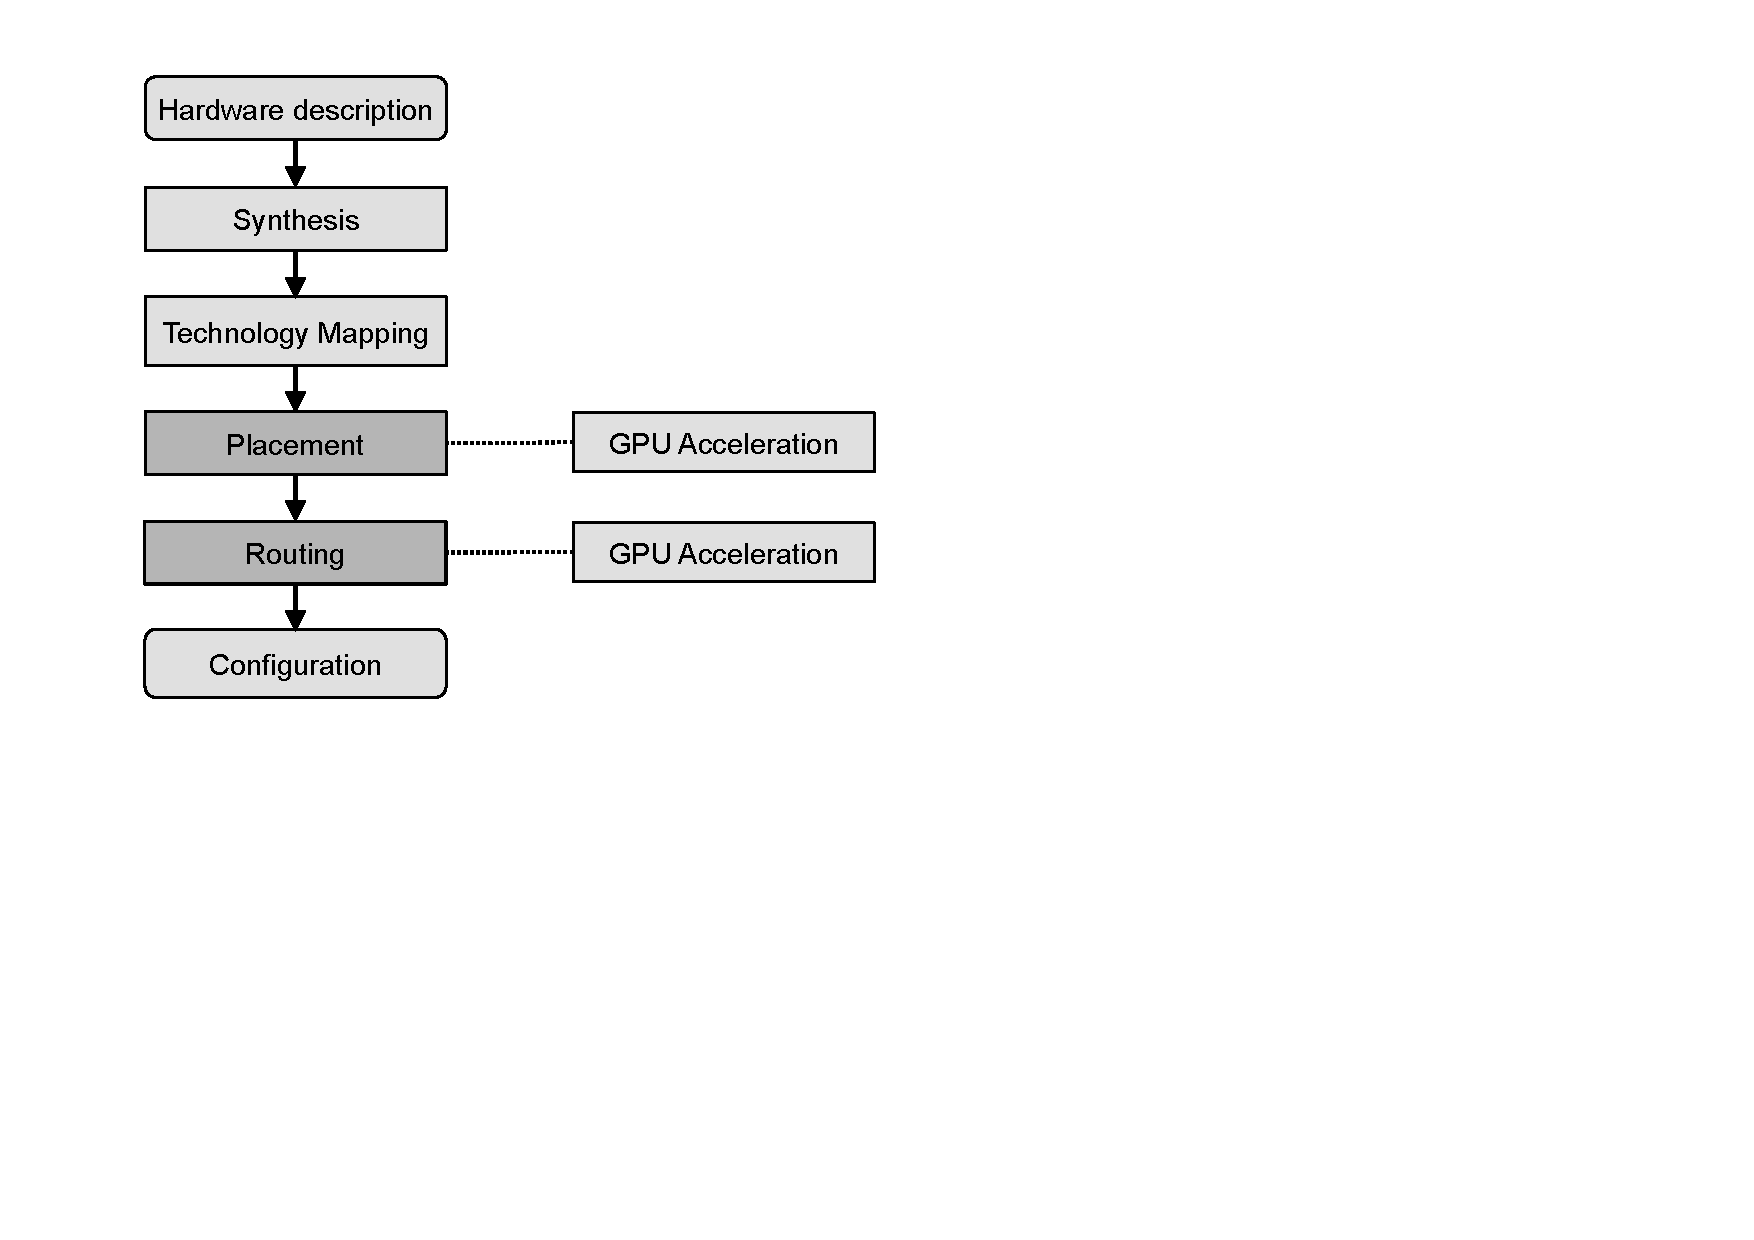
\includegraphics[width = 0.50\textwidth,trim = 0mm 90mm 140mm 2mm, clip]{toolflow}
\caption{Schematic representation of the toolflow. The placement and routing step will be accelerated by a GPU kernel.}
\label{toolflows}
\end{figure}

\subsubsection{Placement techniques}\label{placetech}


\subsubsection{Routing techniques}\label{routetech}

\hl{Routing resource graph
graph based
move away from graph based routing algorithms
tile based
divide and conquer}

\newpage

\section{Timetable \hl{(1 page)}}\label{timetable}
\hl{ Indicate the timeframe for each broad stage considering literature surveys, data collection, production, modelling, review, analysis,
testing, reporting, chapter and thesis writing, and thesis submission date.}

The research in this project will be divided in 2 big stages:

\subsection{Work Packages}
\begin{description*}
\item[Hardware Acceleration of the placement (18 months)]\

\begin{description*}
\item[Adapt the liquid placement algorithm for wide-scale parallelization (9+1 months)]\
In the first step the placer prototype will be further developed and elaborated with the features that were described in the previous section. After this work there is one month allocated for writing a conference paper to report about the initial results.
\item[Implementation of GPU Accelerator for Placement (9+1 months)]\
After developing the placement algorithm, it will be implemented on the GPU. Measurements and results will be reported in another conference paper and a demonstration will be held at one of the workshops accompanying a conference. 
\end{description*}

\item[Hardware Acceleration of the the routing (17 months)]\

\begin{description*}
\item[Exploration new routing algorithms for wide-scale parallelization (8 months)] 
New scalable routing algorithms with 
\item[Implementation of GPU/FPGA accelerator for Routing (9+1 months)]
After developing the routing algorithm, it will be implemented on the GPU/FPGA. Measurements and results will be reported in another conference paper and a demonstration will be held at one of the workshops accompanying a conference. 
\end{description*}

\item[Writing the doctoral thesis and reporting final results. (6 months)] This time is allocated to write the thesis and to report the finalized results in journals and conferences.  

\end{description*}

\begin{figure}[ht]
\centering
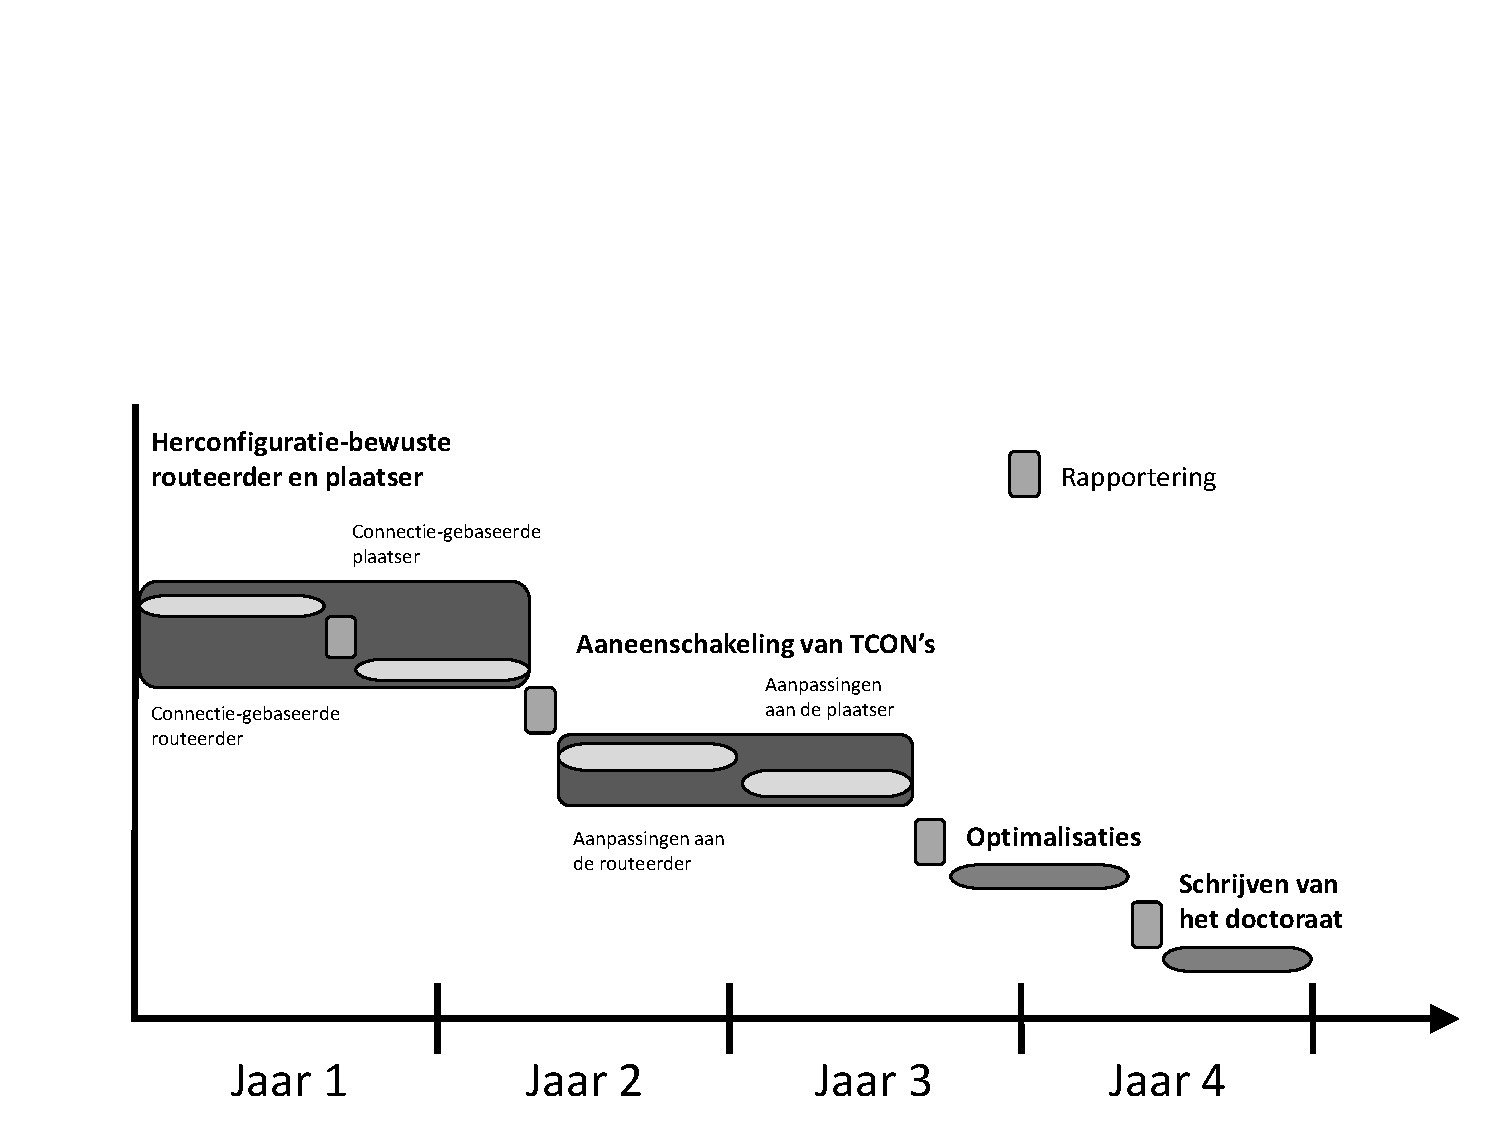
\includegraphics[width = \textwidth,trim = 0mm 0mm 0mm 70mm, clip]{tijdschema.pdf}
\end{figure}

\newpage
\section{Feasibility\hl{(1 page)}}
\hl{Expected outcomes, significance or rationale
Why is it important? 
What do you expect it will deliver? 
What are the expected outcomes? 
Establish the importance of your project by highlighting its originality or why it is worth pursuing. Highlight the benefits, positive expected outcomes or innovative applications of knowledge.}

\hl{Dirk: I can probably write this part after the rest of the proposal is written.}
Elias: Maybe we can tell here that the first stage is less risk and we are more confident that we will succeed here, because we already developed a good base algorithm that will be easier to parallelize, but for the second stage we did not yet devise a new algorithm. So the second stage has inherent more risk because we have yet to start research there.


\subsection{Context and Strategy}\label{context}
My research will be conducted at Ghent University in the research group Hardware and Embedded Systems (HES). HES is part of the Computer Systems Lab (CSL) in the Department of Electronics and Information Systems. The HES group is lead by professor Dirk Stroobandt. The group has a lot of experience with developping FPGA CAD tool software.



\newpage
%\nocite{*}
\bibliographystyle{phdsymp}
\bibliography{proposal} % commented if *.bbl file included, as
%\bibliography{../../../bib/hes} % commented if *.bbl file included, as
%%%%%see below
%%DIrk_bis: in je referenties hoofdletters escapen door ze tussen {} te zetten, zoals voor {FPGA}'s.

%%%%%%%%%%%%%%%%% BIBLIOGRAPHY IN THE LaTeX file !!!!! %%%%%%%%%%%%%%%%%%%%%%%%
%% This is nothing else than the phdsymp_sample2e.bbl file that you would%%
%% obtain with BibTeX: you do not need to send around the *.bbl file        
%%
%%---------------------------------------------------------------------------%%
%
%\begin{thebibliography}{1}
%\bibitem{LaTeX}
%Leslie Lamport,
%\newblock {\em A Document Preparation System: \LaTeX, User's Guide and
%  Reference Manual},
%\newblock Addison Wesley Publishing Company, 1986.
%\bibitem{LaTeXD}
%Helmut Kopka,
%\newblock {\em \LaTeX, eine Einf\"uhrung},
%\newblock Addison-Wesley, 1989.
%\bibitem{TeX}
%D.K. Knuth,
%\newblock {\em The {\rm T\kern-.1667em\lower.7ex\hbox{E}\kern-.125emX}book},
%\newblock Addison-Wesley, 1989.
%\bibitem{METAFONT}
%D.E. Knuth,
%\newblock {\em The {\rm METAFONT}book},
%\newblock Addison Wesley Publishing Company, 1986.
%\end{thebibliography}
%
%%---------------------------------------------------------------------------%%

\end{document}

%%%%%%%%%%%%%%%%%%%%%  End of phdsymp_sample2e.tex  %%%%%%%%%%%%%%%%%%%%%%%%%%%

